\section{Getting data from WINDOW program}\label{getting-data-from-window-program}

The WINDOW program is published from LBNL at \url{http://windows.lbl.gov/software}. More specifics on the program and its details are shown in the Input Output Reference under ``Importing Windows from WINDOW program'' topic.

\subsection{EnergyPlus IDF Excerpt Data}\label{energyplus-idf-excerpt-data}

The preferred method of using WINDOW data in EnergyPlus is to excerpt or ``report'' a specific Window from the Window library screen (see below):

\begin{figure}[hbtp] % fig 1
\centering
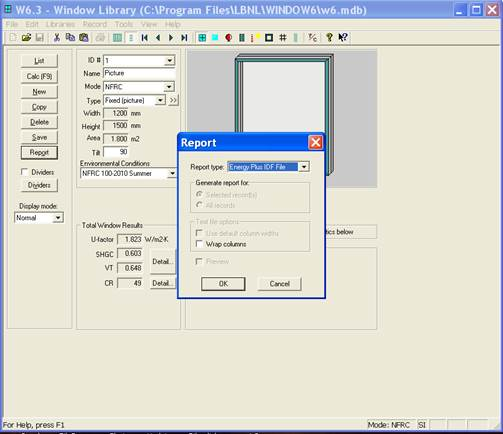
\includegraphics[width=0.9\textwidth, height=0.9\textheight, keepaspectratio=true]{media/image001.jpg}
\caption{WINDOW screen for exporting IDF Window specifications \protect \label{fig:window-screen-for-exporting-idf-window}}
\end{figure}

The file can then be saved at a location of your choice and added into your overall simulation IDF file.

\subsection{WINDOW Data File}\label{window-data-file}

The other ``older'' option for creating data for EnergyPlus is to use the ``EnergyPlus'' option above and create a WindowDataFile. The general format of this data is described in the following paragraphs and must use the Construction:WindowDataFile object and an external file to be used in EnergyPlus. While this is a convenient small file (that can contain multiple windows), there is no way to import this file back into WINDOW and obtain the above, more preferred method.

Please note that there is a bug in WINDOW 5 that causes two of the lines in the EnergyPlus data file to be joined. This bug is fixed in versions of Window 5.02 (and above). To be sure, you can check the data file for a line that looks like:

GLAZING SYSTEM OPTICAL DATAAngle~~~~ 0~~~ 10~~~ 20~~~ 30~~~ 40~~~ 50~~~ 60~~~ 70~~~ 80~~~ 90 Hemis

The fixed version of the program will not show the above line; rather, there will be two lines such as shown below. If you have the above condition, with an editor you would break this into two lines:

GLAZING SYSTEM OPTICAL DATA

Angle~~~~ 0~~~ 10~~~ 20~~~ 30~~~ 40~~~ 50~~~ 60~~~ 70~~~ 80~~~ 90 Hemis

In EnergyPlus, the Window data file is searched for each ``Construction:WindowDataFile'' object in the EnergyPlus input. This object has a very simple form:

Construction:WindowDataFile,

ConstructionName,

FileName; ! Default is Window5DataFile.dat in the ``run'' folder.

If there is a window called ConstructionName on the Window data file, the data for that window is read from the file and the following EnergyPlus objects and their names are created. The ``W5'' prefixed to these names indicates that the object originated in the Window5 data file.

\begin{itemize}
\item
  \textbf{WindowMaterial:Glazing} for each of the glass layers. They will be named \textbf{W5:ConstructionName:GLASS1}, \textbf{W5:ConstructionName:GLASS2} , etc.
\item
  \textbf{WindowMaterial:Gas} or \textbf{WindowMaterial:GasMixture} for each of the gap layers. They will be named \textbf{W5:ConstructionName:GAP1}, \textbf{W5:ConstructionName:GAP2} , etc.
\item
  \textbf{WindowProperty:FrameAndDivider} (if the window on the Window5 data file has a frame and/or divider). It will be named \textbf{W5:ConstructionName}. This WindowProperty:FrameAndDivider will be assigned to any window on the input file that has a construction called ``ConstructionName'' \emph{even if that window has~ referenced another WindowProperty:FrameAndDivider (i.e., if WindowProperty:FrameAndDivider Name for that window is specified).} In this case a warning will result.
\end{itemize}

Note that:

An entry on the WINDOW data file usually has just one glazing system. It is also possible to have an entry with two glazing systems separated by a horizontal or vertical mullion. In this case, the two glazing systems can have different dimensions and different properties. For example, one of the two glazing systems could be single glazed and the other could be double glazed. An example~ of the two glazing system case is given in the sample WINDOW data file shown below (although in this case the properties of the two glazing systems are the same).

EnergyPlus handles the ``one glazing system'' and ``two glazing systems'' cases differently. If there is one glazing system, the glazing system height and width from the Window5 data file are not used. Instead, the window dimensions are obtained from the window vertices that have been specified on the IDF file. However, a warning message will result if the height or width calculated from the window's vertex inputs differs from the corresponding Window5 data file values by more than 10\%. This warning is given since the effective frame and edge-of-glass conductances on the WINDOW data file can depend on the window dimensions if the frame is non-uniform, i.e., consists of sections with different values of width, projection, or thermal properties.

If the WINDOW data file entry has two glazing systems, System1 and System2, the following happens, as shown in the figure below. Assume that the original window is called WinOriginal. System1 is assigned to WinOriginal. Then EnergyPlus automatically creates a second window, called WinOriginal:2, and assigns System2 to it. The dimensions of WinOriginal are ignored; the dimensions of System1 on the data file are assigned to it, but the position of the lower left-hand vertex of WinOriginal is retained. The dimensions of System2 on the data file are assigned to WinOriginal:2. The lower left-hand vertex of WinOriginal:2 is determined from the mullion orientation and width.

\textbf{Note: WinOriginal would have been the IDF window definition -- it's dimensions will be overridden by the systems dimensions from the Window data file. Two windows will be made and called WinOriginal and WinOriginal:2.}

\begin{figure}[hbtp] % fig 2
\centering
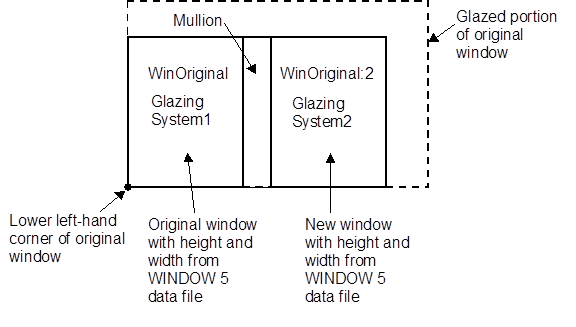
\includegraphics[width=0.9\textwidth, height=0.9\textheight, keepaspectratio=true]{media/image002.png}
\caption{Window Glazing system with dual glazing constructions \protect \label{fig:window-glazing-system-with-dual-glazing}}
\end{figure}

The Window Data File contains no information on shading devices. See ``Specify the Material Name of the Shading Device'' under WindowProperty:ShadingControl for a method to attach a shading layer to windows read in from this file.

Following is an example WINDOW data file for a slider window with two identical double low-E glazing systems separated by a horizontal mullion. Each system has a frame and divider. Note that all dimensions, such as glazing height and width, are in millimeters; when EnergyPlus reads the file these are converted to meters. Following the data file example is a description of the contents of the file. That data used by EnergyPlus is shown in bold.

Window5 Data File for EnergyPlus

\textless{}WINDOW program version\textgreater{}

Date~~~~~~~~~~~~ : Tue Nov 13 17:07:40 2001

Window name~~~~~ : \textbf{DoubleLowE}

Description~~~~~ : Horizontal Slider, AA

\# Glazing Systems: \textbf{2}

GLAZING SYSTEM DATA: Height Width nPanes Uval-center SC-center SHGC-center Tvis-center

~System1~~~~~~~~ :~~ 1032~~ 669~~~~~ 2~~~~~ 1.660~~~~~ 0.538~~~~~ 0.467~~~~~~ 0.696

~System2~~~~~~~~ :~~ 1033~~ 669~~~~~ 2~~~~~ 1.660~~~~~ 0.538~~ ~~~0.467~~~~~~ 0.696

FRAME/MULLION DATA: Width OutsideProj InsideProj Cond EdgeCondRatio SolAbs VisAbs Emiss~ Orient'n (mull)

~~~ L Sill~~~~~~ :~~ 97.3~~~~ 25.4~~~~~~ 25.4~~ 500.000~~~ 1.467~~~~ 0.500~ 0.500~ 0.90

~~~ R Sill~~~~~~ :~~ 97.3~~~~ 25.4~~~~~~ 25.4~~ 500.000~~~ 1.467~~~~ 0.500~ 0.500~ 0.90

~~~ L Head~~~~~~ :~~ 70.2~~~~ 25.4~~~~~~ 25.4~~ 18.822~~~~ 1.490~~~~ 0.500~ 0.500~ 0.90

~~~ R Head~~~~~~ :~~ 70.2~~~~ 25.4~~~~~~ 25.4~~ 18.822~~~~ 1.490~~~~ 0.500~ 0.500~ 0.90

~~~ Top L Jamb~~ :~~ 54.3~~~~ 25.4~~~~~~ 25.4~~ 31.141~~~~ 1.503~~~~ 0.500~ 0.500~ 0.90

~~~ Bot L Jamb~~ :~~ 54.3~~~~ 25.4~~~~~~ 25.4~~ 500.000~~~ 1.494~~~~ 0.500~ 0.500~ 0.90

~~~ Top R Jamb~~ :~~ 70.2~~~~ 25.4~~~~~~ 25.4~~ 500.000~~~ 1.518~~~~ 0.500~ 0.500~ 0.90

~~~ Bot R Jamb~~ :~~ 97.6 ~~~~25.4~~~~~~ 25.4~~ 264.673~~~ 1.547~~~~ 0.500~ 0.500~ 0.90

~~~ Mullion~~~~~ :~~ 53.5~~~~ 25.4~~~~~~ 25.4~~ 500.000~~~ 1.361~~~~ 0.500~ 0.500~ 0.90 \textbf{Horizontal}

~~~ Average frame:~~ \textbf{75.5~~~~ 25.4~~~~~~ 25.4~~ 326.149~~~ 1.464~~~~ 0.500~ 0.500~ 0.90}

DIVIDER DATA~~~~ : Width OutsideProj InsideProj Cond EdgeCondRatio SolAbs VisAbs Emiss Type~~~~~~~~~~~ \#Hor \#Vert

~System1~~~~~~~~ :~ \textbf{25.4~~~ 25.4~~~~~~ 25.4~~~ 3.068~~~~~ 1.191~~~~ 0.500~ 0.500 0.900 DividedLite~~~~~~ 2~~~ 3}

~System2~~~~~~~~ :~ \textbf{25.4~~~ 25.4~~~~ ~~25.4~~~ 3.068~~~~~ 1.191~~~~ 0.500~ 0.500 0.900 DividedLite~~~~~~ 2~~~ 3}

GLASS DATA~~~~~~ : Layer\#~ Thickness~ Cond Tsol Rfsol Rbsol Tvis Rfvis Rbvis~ Tir~ EmissF~ EmissB~ SpectralDataFile

~System1~~~~~~~~ :~~ 1~~~~~ \textbf{3.00~~~~ 0.900} 0.50~ 0.33~ 0.39 0.78~ 0.16~ 0.13 \textbf{0.00~~ 0.16~~~ 0.13}~~ CMFTIR\_3.AFG

~~~~~~~~~~~~~~~~~~~~ 2~~~~~ \textbf{6.00~~~~ 0.900} 0.77~ 0.07~ 0.07 0.88~ 0.08~ 0.08 \textbf{0.00~~ 0.84~~~ 0.84}~~ CLEAR\_6.DAT

~System2~~~~~~~~ :~~ 1~~~~~ \textbf{3.00~~~~ 0.900} 0.50~ 0.33~ 0.39 0.78~ 0.16~ 0.13 \textbf{0.00~~ 0.16~~~ 0.13}~~ CMFTIR\_3.AFG

~~~~~~~~~~~~~~~~~~~~ 2~~~~~ \textbf{6.00~~~~ 0.900} 0.77~ 0.07~ 0.07 0.88~ 0.08~ 0.08 \textbf{0.00~~ 0.84~~~ 0.84}~~ CLEAR\_6.DAT

GAP DATA~~~~~~~~ : Gap\# Thick nGasses

~System1~~~~~~~~ :~~ 1~ \textbf{12.70~~~ 1}

~System2~~~~~~~~ :~~ 1~ \textbf{12.70~~~ 1}

GAS DATA~~~~~~~~ : GasName Fraction MolWeight ACond~~ BCond~ CCond AVisc~~ BVisc~~ CVisc ASpHeat~ BSpHeat CSpHeat

~System1 Gap1~~~ : Air~~~~ \textbf{1.0000~~ 28.97~~~ 0.002873 7.76e-5 0.0 3.723e-6 4.94e-8 0.0~~ 1002.737 0.012324 0.0}

~System2 Gap1~~~ : Air~~~~ \textbf{1.0000~~ 28.97~~~ 0.002873 7.76e-5 0.0 3.723e-6 4.94e-8 0.0~~ 1002.737 0.012324 0.0}

GLAZING SYSTEM OPTICAL DATA

Angle~~~~ 0~~~ 10~~~ 20~~~ 30~~~ 40~~~ 50~~~ 60~~~ 70~~~ 80~~~ 90 Hemis

System1

Tsol~ \textbf{0.408 0.410 0.404 0.395 0.383 0.362 0.316 0.230 0.106 0.000 0.338}

Abs1~ \textbf{0.177 0.180 0.188 0.193 0.195 0.201 0.218 0.239 0.210 0.001 0.201}

Abs2~ \textbf{0.060 0.060 0.061 0.061 0.063 0.063 0.061 0.053 0.038 0.000 0.059}

Rfsol \textbf{0.355 0.350 0.348 0.350 0.359 0.374 0.405 0.478 0.646 0.999 0.392}

Rbsol \textbf{0.289 0.285 0.283 0.282 0.285 0.296 0.328 0.411 0.594 1.000 0.322}

Tvis~ \textbf{0.696 0.700 0.690 0.677 0.660 0.625 0.548 0.399 0.187 0.000 0.581}

Rfvis \textbf{0.207 0.201 0.198 0.201 0.212 0.234 0.278 0.374 0.582 0.999 0.260}

Rbvis \textbf{0.180 0.174 0.173 0.176 0.189 0.215 0.271 0.401 0.648 1.000 0.251}

System2

Tsol~ \textbf{0.408 0.410 0.404 0.395 0.383 0.362 0.316 0.230 0.106 0.000 0.338}

Abs1~ \textbf{0.177 0.180 0.188 0.193 0.195 0.201 0.218 0.239 0.210 0.001 0.201}

Abs2~ \textbf{0.060 0.060 0.061 0.061 0.063 0.063 0.061 0.053 0.038 0.000 0.059}

Rfsol \textbf{0.355 0.350 0.348 0.350 0.359 0.374 0.405 0.478 0.646 0.999 0.392}

Rbsol \textbf{0.289 0.285 0.283 0.282 0.285 0.296 0.328 0.411 0.594 1.000 0.322}

Tvis~ \textbf{0.696 0.700 0.690 0.677 0.660 0.625 0.548 0.399 0.187 0.000 0.581}

Rfvis \textbf{0.207 0.201 0.198 0.201 0.212 0.234 0.278 0.374 0.582 0.999 0.260}

Rbvis \textbf{0.180 0.174 0.173 0.176 0.189 0.215 0.271 0.401 0.648 1.000 0.251}

\textbf{Description of Contents of WINDOW Data File}

(Quantities used in EnergyPlus are in bold; others are informative only)

Second line = version of WINDOW used to create the data file

\emph{Date} = date the data file was created

\textbf{\emph{Window name}} = name of this window; chosen by WINDOW5 user; EnergyPlus user enters the same name in EnergyPlus as name of a ``Construction from Window5 Data File'' object. EnergyPlus will search the Window5 data file for an entry of this name.

\emph{Description} = One-line description of the window; this is treated as a comment.

\textbf{\emph{\# Glazing Systems}}: 1 or 2; value is usually 1 but can be 2 if window has a horizontal or vertical mullion that separates the window into two glazing systems that may or may not be different.

GLAZING SYSTEM DATA

\emph{System1, System2}: separate characteristics given if window has a mullion.

\textbf{\emph{Height}}, *\textbf{\emph{width}} = height and width of glazed portion (i.e., excluding frame; and, if mullion present, excluding mullion).

\textbf{\emph{nPanes}}~~~~ = number of glass layers

\emph{Uval-center} = center-of-glass U-value (including air films) under standard winter conditions*~ (W/m2)

\emph{SC-center}~~ = center-of-glass shading coefficient under standard summer conditions*.

\emph{SHCG-center} = center-of-glass solar heat gain coefficient under standard summer conditions*.

\emph{Tvis-center} = center-of-glass visible transmittance at normal incidence

FRAME/MULLION DATA

\emph{L,R Sill}~~ = left, right sill of frame

\emph{L,R Head}~~ = left, right header of frame

\emph{Top L, Bot L jamb} = top-left, bottom-left jamb of frame

\emph{Bot L, Bot R jamb} = bottom-left, bottom-right jamb of frame

\textbf{\emph{Average frame}} = average characteristics of frame for use in EnergyPlus calculation. If mullion is present, original window is divided into two separate windows with the same average frame (with the mullion being split lengthwise and included in the average frame).

\textbf{\emph{Width}}~~~~ = width (m)

\textbf{\emph{OutsideProj}} = amount of projection from outside glass (m)

\textbf{\emph{InsideProj}} = amount of projection from inside glass (m)

\textbf{\emph{Cond}} = effective surface-to-surface conductance (from THERM calculation) (W/m2)

\textbf{\emph{EdgeCondRatio}} = ratio of surface-to-surface edge-of-glass conductance to surface-to-surface center-of-glass conductance (from THERM calculation)

\textbf{\emph{SolAbs}}~~~ = solar absorptance

\textbf{\emph{VisAbs}}~~~ = visible absorptance

\textbf{\emph{Emiss}}~~~~ = hemispherical thermal emissivity

\textbf{\emph{Orientation}} = Horizontal or Vertical (mullion only); = None if no mullion.

DIVIDER DATA

\textbf{\emph{Width}} through \textbf{\emph{Emiss}} are the same as for FRAME/MULLION DATA

\textbf{\emph{\#Hor}}~~~~~ = number of horizontal dividers

\textbf{\emph{\#Vert}}~~~~ = number of vertical dividers

\textbf{\emph{Type}}~~~~~ = DividedLite or Suspended

GLASS DATA

\emph{System1, System2}: separate characteristics are given if window has a mullion.

\textbf{\emph{Cond}}~~~~~~ = conductivity (W/m-K)

\emph{Tsol}~~~~~~ = spectral-average solar transmittance at normal incidence

\emph{Rfsol}~~~~~ = spectral-average front solar reflectance at normal incidence

\emph{Rbsol}~~~~~ = spectral-average back solar reflectance at normal incidence

\emph{Tvis}~~~~~~ = spectral-average visible transmittance at normal incidence

\emph{Rfvis}~~~~~ = spectral-average front visible reflectance at normal incidence

\emph{Rbvis}~~~~~ = spectral-average back visible reflectance at normal incidence

\textbf{\emph{Tir}}~~~~~~ = hemispherical IR transmittance

\textbf{\emph{EmissF}}~~~ = hemispherical front emissivity

\textbf{\emph{EmissB}}~~~ = hemispherical back emissivity

SpectralDataFile = name of spectral data file with wavelength-dependent transmission and reflection data used by WINDOW 5 to calculate the glazing system optical data. ``None'' will appear here if spectral-average data for this glass layer were used by WINDOW 5.

GAP DATA

System1, System2: separate characteristics are given if the window has a mullion.

\textbf{\emph{Thick}}~~~~ = thickness (m)

\textbf{\emph{nGasses}}~ = number of gasses (1, 2 or 3)

GasName~~ = name of the gas

\textbf{\emph{Fraction}}~ = fraction of the gas

\textbf{\emph{MolecWeight}} = molecular weight of the Nth gas

(In the following, conductivity, viscosity and specific heat as a function

of temperature, T (deg K), are expressed as A + B*T + C*T\^{}2)

\textbf{\emph{ACond}}~~~~ = A coeff of conductivity (W/m-K)

\textbf{\emph{BCond}}~~~~ = B coeff of conductivity (W/m-K\^{}2)

\textbf{\emph{CCond}}~~~~ = C coeff of conductivity (W/m-K\^{}3)

\textbf{\emph{AVisc}}~~~~ = A coeff of viscosity (g/m-s)

\textbf{\emph{BVisc}}~~~~ = B coeff of viscosity (g/m-s-K)

\textbf{\emph{CVisc}}~~~~ = C coeff of viscosity (g/m-s-K\^{}2)

\textbf{\emph{ASpHeat}}~~ = A coeff of specific heat (J/kg-K)

\textbf{\emph{BSpHeat}}~~ = B coeff of specific heat (J/kg-K\^{}2)

\textbf{\emph{CSpHeat}}~~ = C coeff of specific heat (J/kg-K\^{}3)

GLAZING SYSTEM OPTICAL DATA

System1, System2: separate characteristics are given if the window has a mullion.

\textbf{\emph{Hemisph}}~~ = hemispherical (i.e., diffuse)

\textbf{\emph{Tsol}}~~~~~ = solar transmittance vs.~angle of incidence

\textbf{\emph{AbsN}}~~~~~ = solar absorptance of Nth layer vs.~angle of incidence

\textbf{\emph{Rfsol}}~~~~ = front solar reflectance vs.~angle of incidence

\textbf{\emph{Rbsol}}~~~~ = back solar reflectance vs.~angle of incidence

\textbf{\emph{Tvis}}~~~~~ = visible transmittance vs.~angle of incidence

\textbf{\emph{Rfvis}}~~~~ = front visible reflectance vs.~angle of incidence

\textbf{\emph{Rbvis}}~~~~ = back visible reflectance vs.~angle of incidence

\begin{center}\rule{0.5\linewidth}{\linethickness}\end{center}

*Standard conditions are

~ Winter:

~ Indoor air temperature = 21.1C (70F)

~ Outdoor air temperature = -17.8C (0F)

~ Wind speed = 6.71 m/s (15 mph)

~ No solar radiation

~ Summer:

~ Indoor air temperature = 23.9C (75F)

~ Outdoor air temperature = 31.7C (89F)

~ Wind speed = 3.35 m/s (7.5 mph)

~ 783 W/m2 (248 Btu/h-ft2) incident beam solar radiation normal to glazing
